\section{Background}
\begin{frame}[fragile]
\frametitle{\insertsection}
\end{frame}

\section[\arara]{\arara}

\subsection{¿Qué es esta herramienta?}

\begin{frame}
\frametitle{\insertsection}
\begin{block}{\insertsubsection}
	\begin{itemize}
		\item Herramienta de automatización \TeX{} basada en reglas y directivas.
		\item Control de los documentos: \arara\ no hará algo a menos que le enseñes la tarea y le digas explícitamente la tarea a ejecutar.
	\end{itemize}
\end{block}
\end{frame}

\subsection{Conceptos claves}

\begin{frame}
\frametitle{\insertsection}
\begin{block}{\insertsubsection}
\begin{itemize}
	\item Reglas: Descripción formal de cómo \arara\ maneja una determinada tarea.
	\item Directivas: Comentario especial que se inserta en el código fuente en el que le indicas cómo \arara\ debería comportarse.
	\item Ejemplos de directivas: \texttt{latex}, \texttt{xelatex}, \texttt{luatex}, \texttt{clean}, \texttt{indent}. \texttt{make}, \texttt{xindy}, \texttt{makeglossaries}, incluso puedes crear tus propias directivas.
\end{itemize}
\end{block}
\end{frame}

\subsection{Algunos métodos}

\begin{frame}
\frametitle{\insertsection}
\begin{block}{\insertsubsection}

\end{block}
\end{frame}

\subsection{Cajas de diálogo}

\begin{frame}
\frametitle{\insertsection}
\begin{block}{\insertsubsection}
Es un elemento de control gráfico, generalmente una pequeña ventana, que comunica información al usuario y le solicita una respuesta.
\end{block}
\end{frame}

\begin{frame}[fragile]
\frametitle{\insertsection}
\begin{codebox}{Terminal}{teal}{\icnote}{white}
$ arara hello.tex 
__ _ _ __ __ _ _ __ __ _ 
/ _` | '__/ _` | '__/ _` |
| (_| | | | (_| | | | (_| |
\__,_|_|  \__,_|_|  \__,_|

Processing 'hello.tex' (size: 86 bytes, last modified: 05/03/2018
07:28:30), please wait.

(PDFLaTeX) PDFLaTeX engine .............................. SUCCESS

Total: 0.73 seconds
\end{codebox}
\end{frame}

\section{Sage}
\subsection{Un programa Sage con variables}

\begin{frame}
\frametitle{\insertsection}
\begin{block}{\insertsubsection}
\begin{itemize}
\item Es un sistema computarizado algebraico.
\item Utiliza el lenguaje de propósito general Python.
\item Creado por el matemático de la Universidad de Washington, William Stein, en el año 2005.
\item Sage reutiliza software libre existentes, algunos de ellos son GAP, PARI-GP, Maxima y Singular.
\item Está escrito completamente en Python.
\end{itemize}
\end{block}
\end{frame}

\begin{frame}[fragile]
\frametitle{\insertsection}
\begin{block}{\insertsubsection}
\begin{sageblock}
f(x) = exp(x) * sin(2*x)
\end{sageblock}
The second derivative of $f$ is

\[
\frac{\mathrm{d}^{2}}{\mathrm{d}x^{2}} \sage{f(x)} =
\sage{diff(f, x, 2)(x)}.
\]

Here's a plot of $f$ from $-1$ to $1$:
\end{block}

\begin{sagesilent}
plt  = plot(f, -1, 1)
plt.save("MyPic.pdf")
\end{sagesilent}

\begin{figure}
\centering
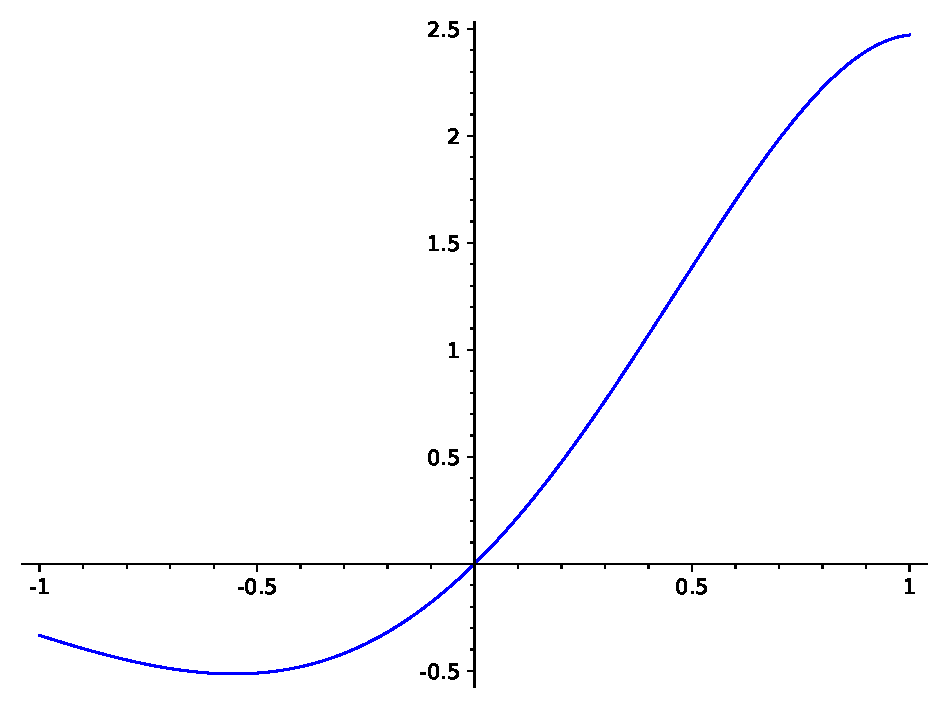
\includegraphics[height=3cm]{MyPic.pdf}
\end{figure}

\end{frame}

\begin{frame}
\begin{block}{Modelo matemático}
Nuestro primer ejemplo se refiere a la programación de un modelo matemático que predice la posición de una pelota lanzada al aire. De la segunda ley de Newton, y asumiendo que la resistencia del aire es insignificante, se puede derivar un modelo matemático que predice la posición $y$ de la pelota en el tiempo $t$.
\end{block}

La declaración $v_0$ = $5$ se llama \emph{asignación}
\end{frame}